

\documentstyle[color,subfigure,graphicx,epsf,here,cite,otf,comment,nccmath,mediabb,fancyhdr,12pt]{jarticle}


\graphicspath{{./pic/}}
%%%\documentstyle{jarticle}
\setlength{\textwidth}{16.2cm}%A4
\setlength{\textheight}{23cm}%A4
\setlength{\topmargin}{-1.5cm}
\setlength{\oddsidemargin}{0cm}
\setlength{\evensidemargin}{0cm}
\setlength{\parskip}{1pt}
%\pagestyle{myheadings}
\pagestyle{fancy}
\lhead[名前]{名前}
\rhead[令和3年4月15日]{令和3年4月15日}
\title{新人ゼミ課題}
\author{大場 大輔}
\date{令和3年4月15日}

\begin{document}
	
	\maketitle
	\vspace*{20pt}

	
\section*{3.時系列識別}
すでに画像処理やPythonを用いたプログラミングの経験があること、Brian先生に配属されたことを考慮して、このコースを選択しました。

\subsection*{動的時間伸縮法について}
動的時間伸縮法(DTW; Dynamic Time Warping)とは、2つの時系列データの距離(類似度)を求める手法であり、具体的には比較するデータの各サンプル同士の(ユークリッド?)距離を総当りで求めて、この2つの



%file:///home/daisuke/Downloads/IPSJ-TOD4504005.pdf
%https://qiita.com/hcpmiyuki/items/251586526c5924f09aa3

\subsection*{Level1}


\begin{figure}[h]
 \begin{minipage}[b]{0.32\linewidth}
  \centering
  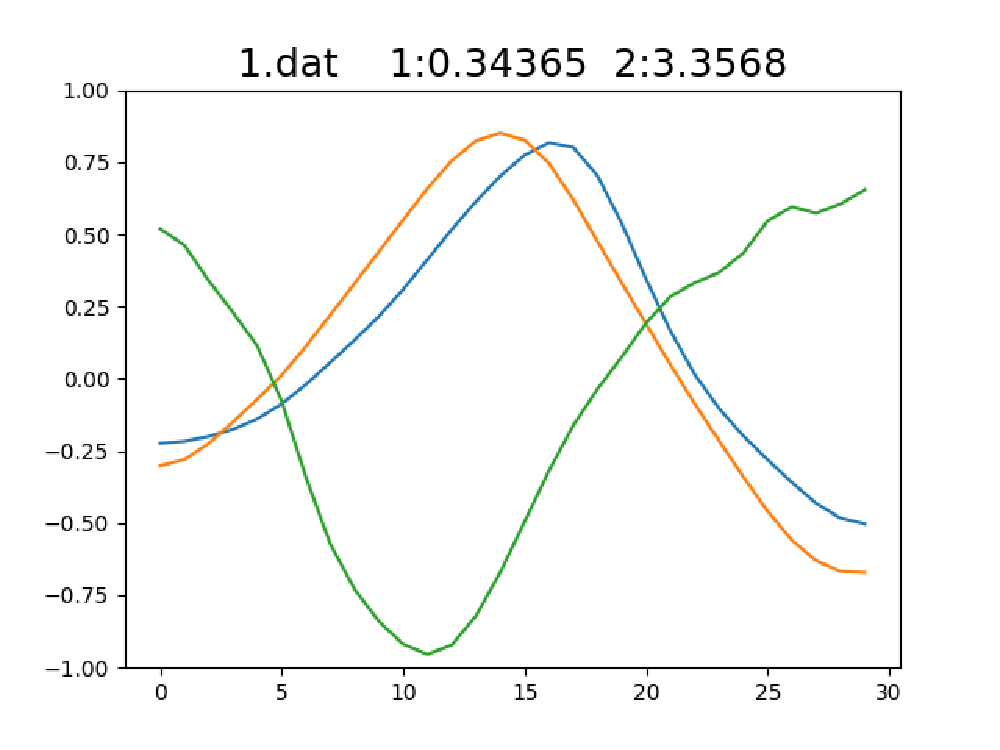
\includegraphics[keepaspectratio, scale=0.3]
  {./pic/level1/1_dat.pdf}
  \label{1dat}
 \end{minipage}
 \begin{minipage}[b]{0.32\linewidth}
  \centering
  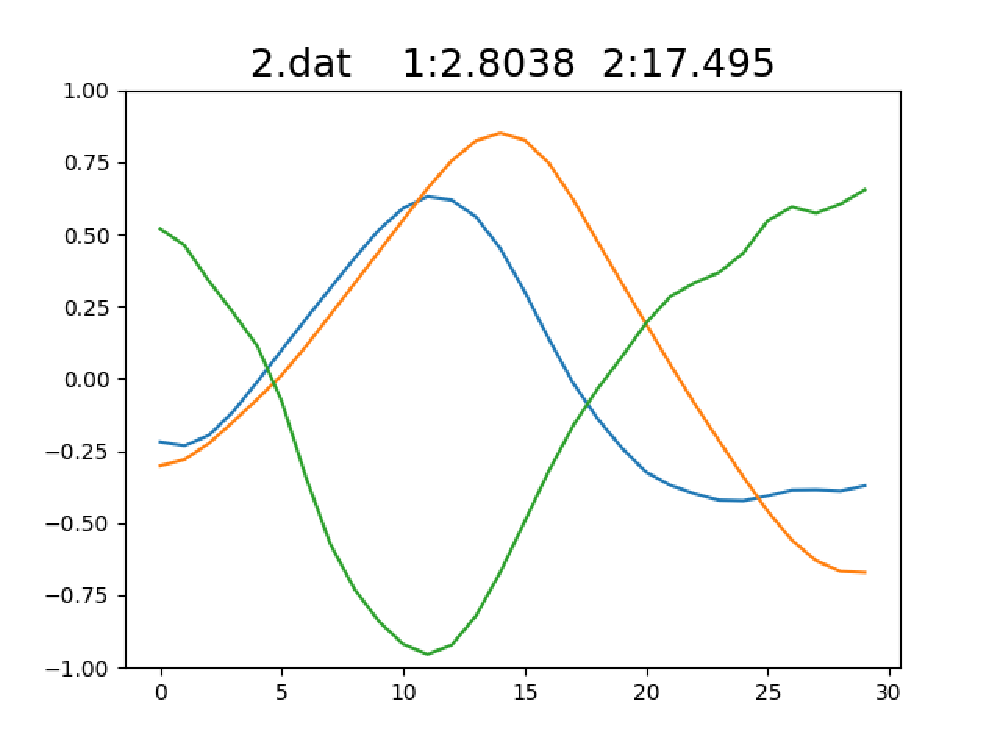
\includegraphics[keepaspectratio, scale=0.3]
  {./pic/level1/2_dat.pdf}
  \label{2dat}
 \end{minipage}
 \begin{minipage}[b]{0.32\linewidth}
  \centering
  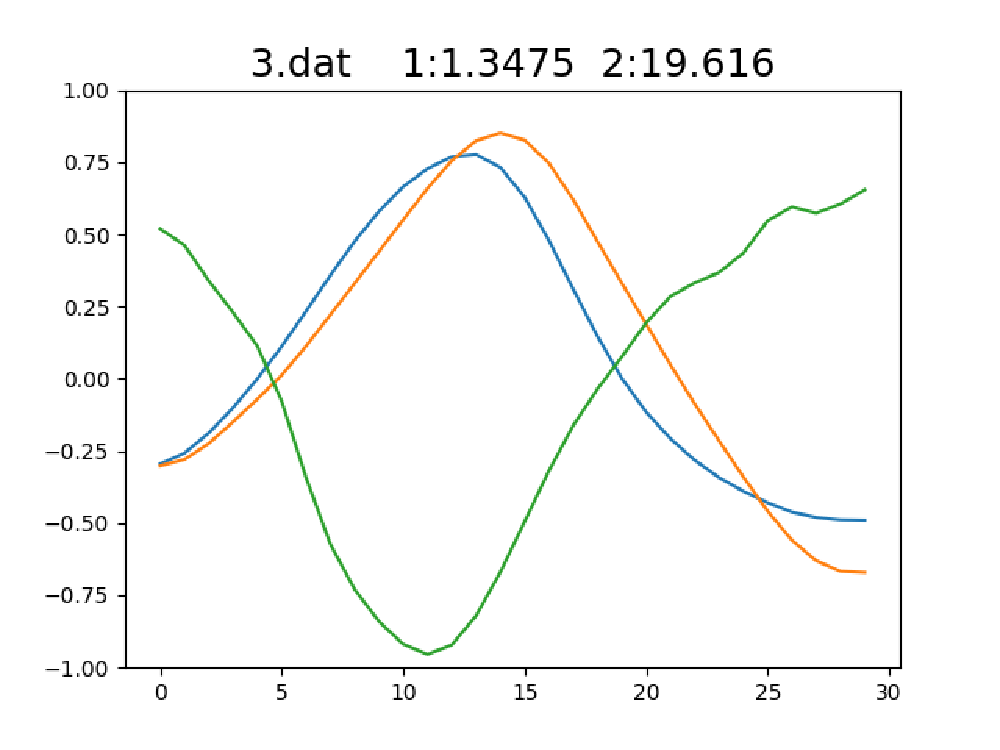
\includegraphics[keepaspectratio, scale=0.3]
  {./pic/level1/3_dat.pdf}
  \label{3dat}
 \end{minipage}\\
 \begin{minipage}[b]{0.32\linewidth}
  \centering
  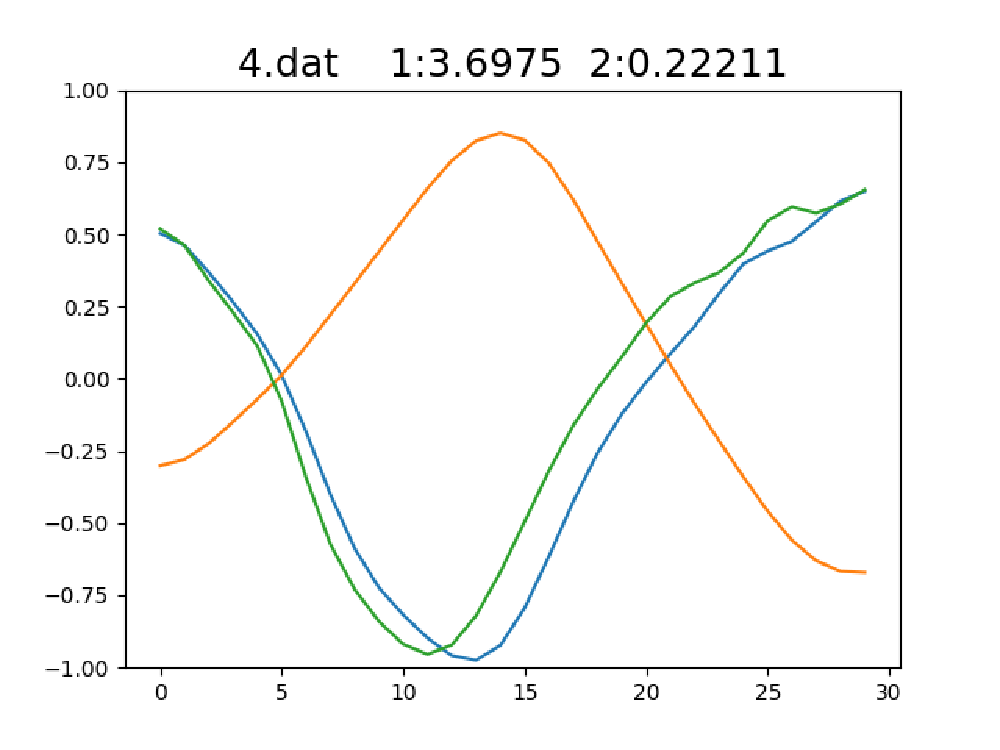
\includegraphics[keepaspectratio, scale=0.3]
  {./pic/level1/4_dat.pdf}
  \label{4dat}
 \end{minipage}
 \begin{minipage}[b]{0.32\linewidth}
  \centering
  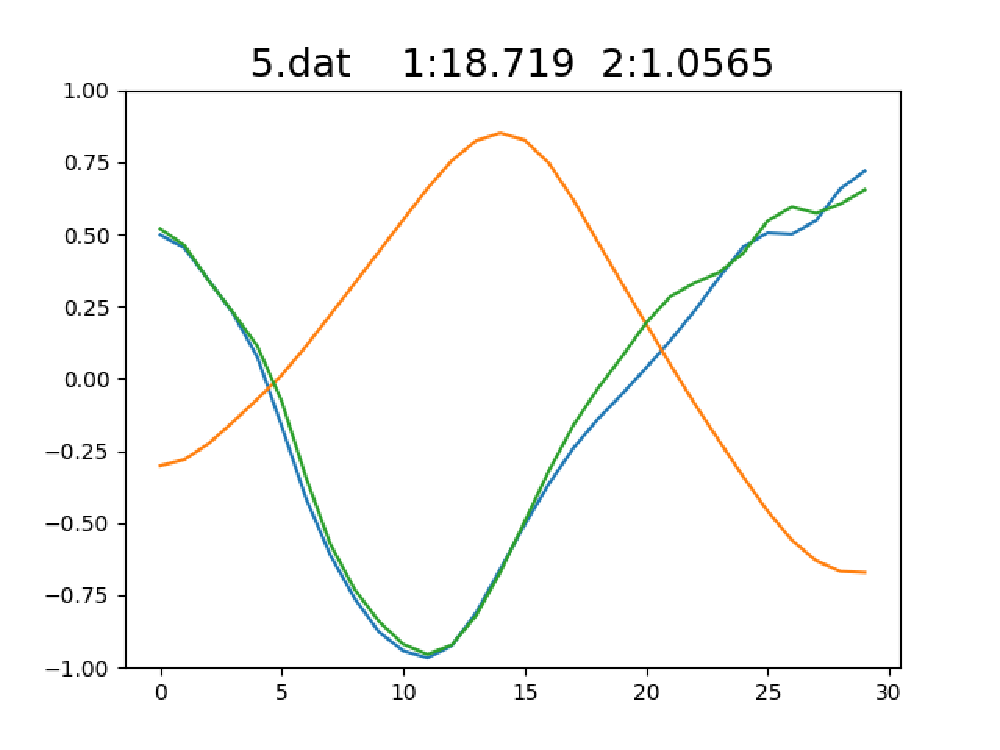
\includegraphics[keepaspectratio, scale=0.3]
  {./pic/level1/5_dat.pdf}
  \label{5dat}
 \end{minipage}
  \begin{minipage}[b]{0.32\linewidth}
  \centering
  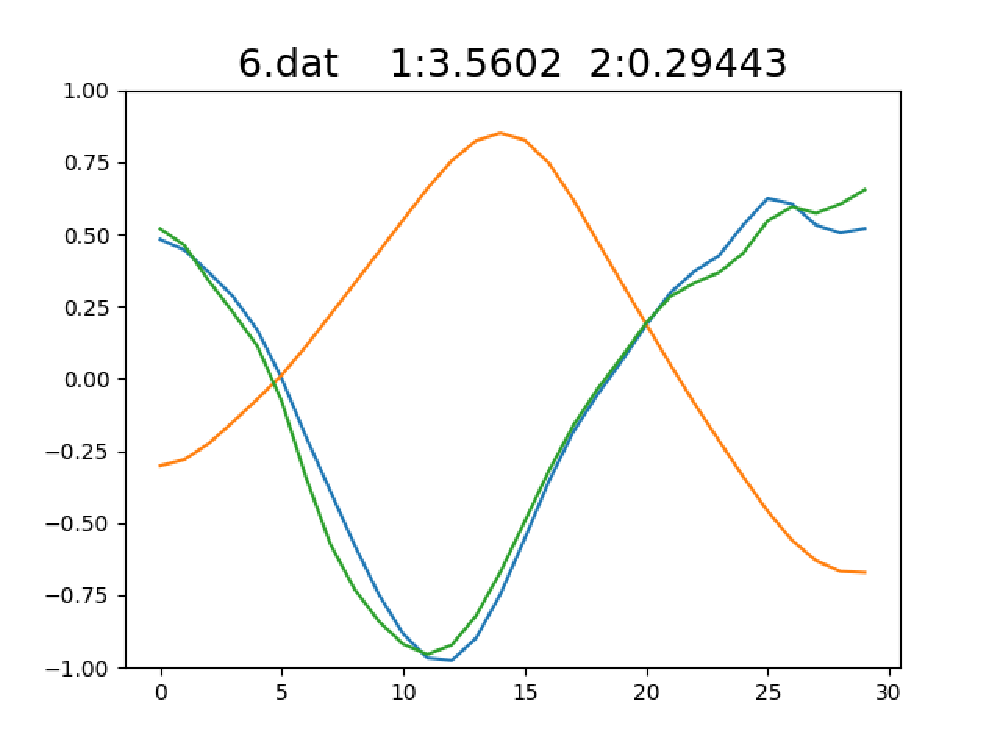
\includegraphics[keepaspectratio, scale=0.3]
  {./pic/level1/6_dat.pdf}
  \label{6dat}
 \end{minipage}
 \caption{各referenceのグラフ。青線が評価対象で、オレンジ線がクラス1、緑線がクラス2を示しています。}\label{reg_poly}
\end{figure}

\subsection*{Level2}

\subsection*{Level3}

\subsection*{Level4}
	
	
	
	
\end{document}
